In this section it is detailed which component is implemented in every stage of the
development process and how the different components are implemented and tested.

\subsubsection*{[F1] Student and Company Registration}
Allows students and companies to register on the platform.

\begin{figure}[h]
    \centering
    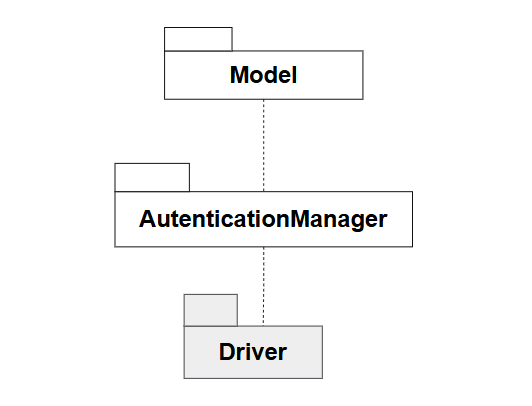
\includegraphics[width=0.5\linewidth]{DD-Latex//assets//Component Integration Graphs/component1.png}
    \caption{Student and Company Registration}
    %\label{fig:enter-label}
\end{figure}

\subsubsection*{[F2] Internship Advertisement Creation and Management}
Verified company users can create, edit, and delete internship advertisements.
Incorporates AI-generated suggestions to improve ad quality (if you choose to utilize RecommendationManager).

\begin{figure}[h]
    \centering
    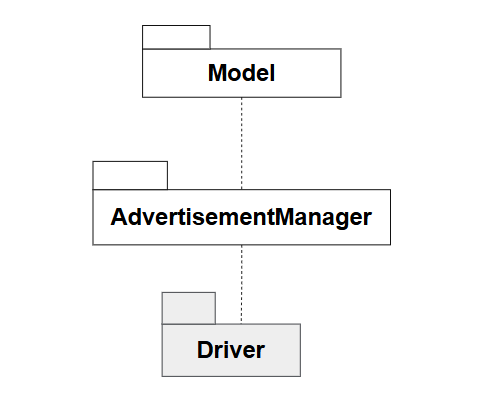
\includegraphics[width=0.5\linewidth]{DD-Latex//assets//Component Integration Graphs/component2.png}
    \caption{Internship Advertisement Creation and Management}
    %\label{fig:enter-label}
\end{figure}

\subsubsection*{[F3] Internship Search and Application}
Students can search available internship ads and apply directly through the platform.
The system recommends internships based on the student’s profile and qualifications.
Once a student applies, their application is recorded, and the company is notified.

\begin{figure}[h]
    \centering
    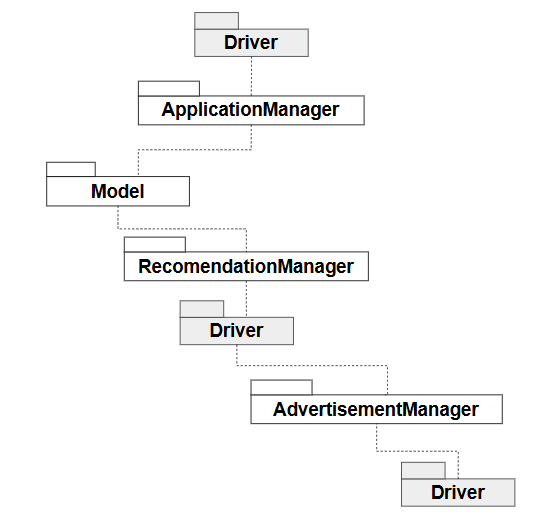
\includegraphics[width=0.5\linewidth]{DD-Latex//assets//Component Integration Graphs/component3.png}
    \caption{Internship Search and Application}
    %\label{fig:enter-label}
\end{figure}

\subsubsection*{[F4] Internship Monitoring and Complaint Management}
Allows students, companies, and universities to monitor ongoing internships.
Users can file a complaint if issues arise.

\begin{figure}[h]
    \centering
    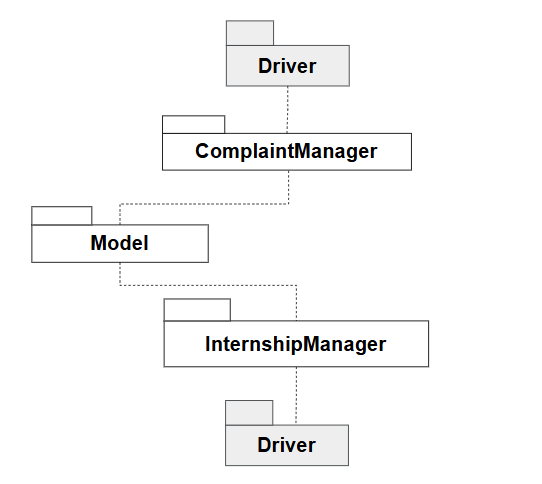
\includegraphics[width=0.5\linewidth]{DD-Latex//assets//Component Integration Graphs/component4.png}
    \caption{Internship Monitoring and Complaint Management}
    %\label{fig:enter-label}
\end{figure}

\subsubsection*{[F5] Feedback Collection and Profile Integration}
Collects feedback from students, companies, and potentially universities after an internship ends.

\begin{figure}[h]
    \centering
    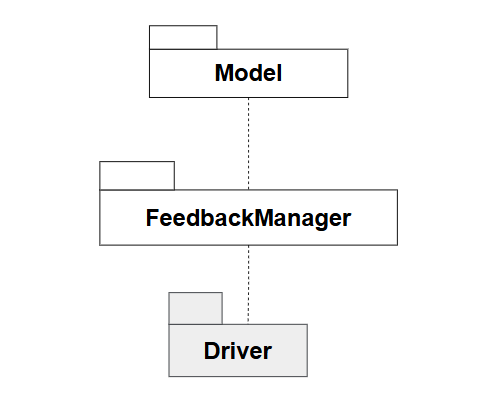
\includegraphics[width=0.5\linewidth]{DD-Latex//assets//Component Integration Graphs/component5.png}
    \caption{Feedback Collection and Profile Integration}
    %\label{fig:enter-label}
\end{figure}